\documentclass[11pt,a4paper]{article}
\usepackage{graphicx}
\usepackage{listings}
\usepackage{hyperref}
\hypersetup{
    colorlinks,
    citecolor=black,
    filecolor=black,
    linkcolor=black,
    urlcolor=black
}
\usepackage{xcolor}
\lstset{basicstyle=\ttfamily,
  showstringspaces=false,
  commentstyle=\color{red},
  keywordstyle=\color{blue}
}
\usepackage{float}
\title{Understandig the Galois Counter Mode (GCM) \\ HW3 - CNS Sapienza}

\author{Edoardo Puglisi 1649359} 
\date{04/11/2019}

\begin{document}
\lstset{breaklines=true}
	
\maketitle
\tableofcontents
\clearpage

\section{Overview}
The following experiment consists of evalutating GCM encryption and decryption speed on binary and text files.

\section{Code}
Code description.
\lstinputlisting[language=bash]{script-hw3-1649359.sh}
This code simply encrypt and decrypt files of different size (text and binary). The process is repeated multiple times for each file to have an average time speed.


\section{Results}
\begin{figure}[H]
    \centering
        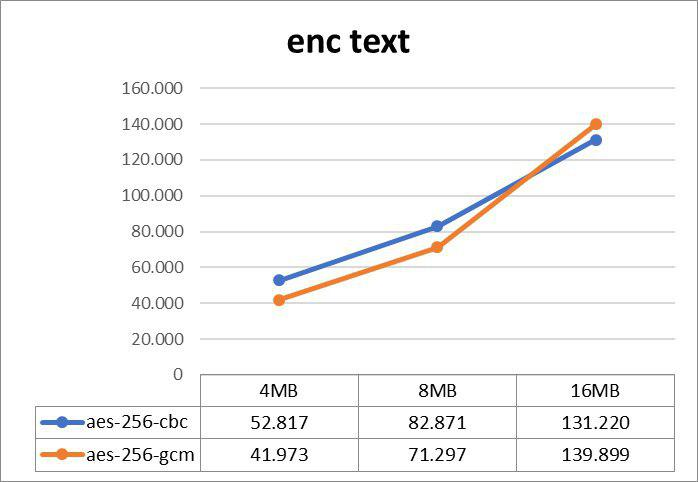
\includegraphics[width=\textwidth]{et-hw3-1649359.jpg}
\end{figure}
\begin{figure}[H]
    \centering
        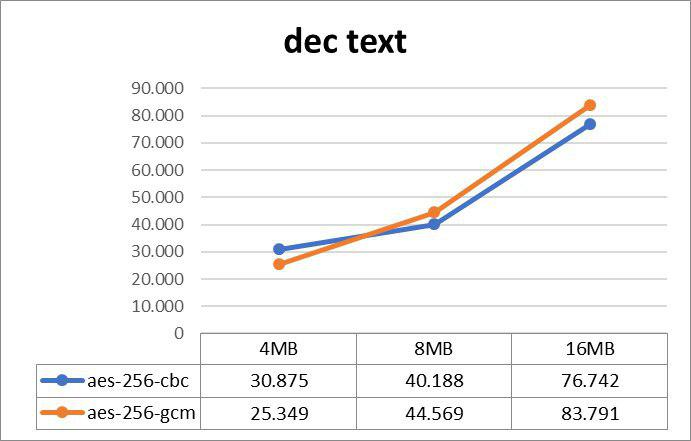
\includegraphics[width=\textwidth]{dt-hw3-1649359.jpg}
\end{figure}

GCM and CBC have almost the same behaviour on text files (GCM a bit slower for grater ones).

\begin{figure}[H]
    \centering
        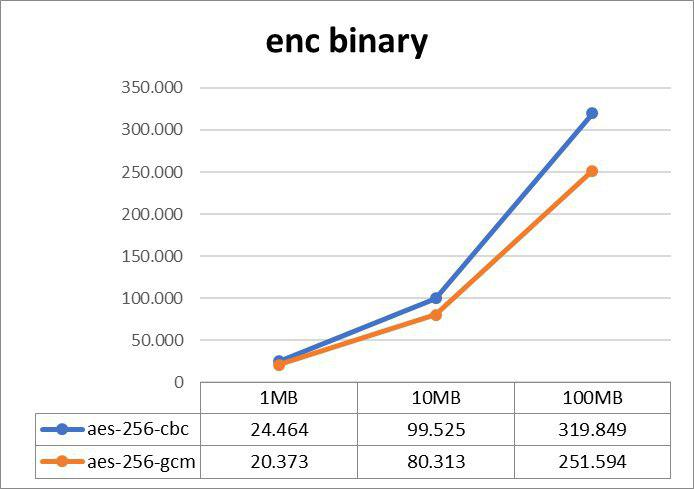
\includegraphics[width=\textwidth]{eb-hw3-1649359.jpg}
\end{figure}
\begin{figure}[H]
    \centering
        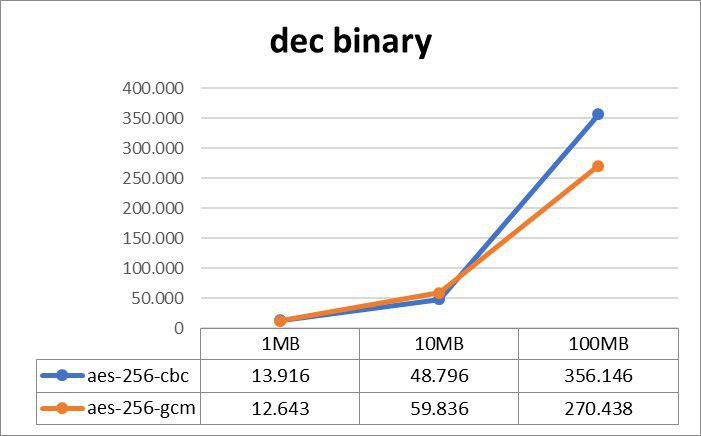
\includegraphics[width=\textwidth]{db-hw3-1649359.jpg}
\end{figure}

For binary files instead the greater is the file, the greater is the difference between GCM and CBC where GCM is much faster.


\end{document}
